
\documentclass[
11pt, % Set the default font size, options include: 8pt, 9pt, 10pt, 11pt, 12pt, 14pt, 17pt, 20pt
%t, % Uncomment to vertically align all slide content to the top of the slide, rather than the default centered
%aspectratio=169, % Uncomment to set the aspect ratio to a 16:9 ratio which matches the aspect ratio of 1080p and 4K screens and projectors
]{beamer}

\graphicspath{{Images/}{./}} % Specifies where to look for included images (trailing slash required)

\usepackage{todonotes}
\usepackage{graphicx}
\usepackage{xcolor}
\usepackage{subfig}
%%\usepackage[noend]{algpseudocode}


\usepackage{algorithm}
\usepackage{algorithmic}

\usepackage{blkarray}
\usepackage{amsmath}
\usepackage{xspace}
\usepackage{float}


\usepackage{tikz}
\usetikzlibrary{matrix, decorations, patterns, positioning, shapes, calc, intersections, arrows, fit}

\usetikzlibrary{patterns}
\usetikzlibrary{fit,calc,positioning,decorations.pathreplacing,matrix,3d, hobby}

%, , 3d, hobby

\usepackage{booktabs} % Allows the use of \toprule, \midrule and \bottomrule for better rules in tables


\newcommand{\brown}[1]{{\color{brown} #1 }}

%% Colors from https://latexcolor.com/
\definecolor{pastelviolet}{rgb}{0.8, 0.6, 0.79}
\definecolor{babyblueeyes}{rgb}{0.63, 0.79, 0.95}
\definecolor{pastelyellow}{rgb}{0.99, 0.99, 0.59}
\definecolor{pastelgreen}{rgb}{0.47, 0.87, 0.47}
\definecolor{pastelred}{rgb}{1.0, 0.41, 0.38}
\colorlet{patternblue}{blue!60}


\colorlet{darkred}{red!80!black}
\colorlet{darkblue}{blue!80!black}
\newcommand<>{\darkred}[1]{{\color{darkred}{#1}}}
\newcommand<>{\darkblue}[1]{{\color#2{blue!50!black!100}{#1}}}

\usetheme{Madrid}





%----------------------------------------------------------------------------------------
%	PRESENTATION INFORMATION
%----------------------------------------------------------------------------------------

\title[Matrix multiplication]{Communication costs of sequential matrix multiplications} % The short title in the optional parameter appears at the bottom of every slide, the full title in the main parameter is only on the title page

%\subtitle{Optional Subtitle} % Presentation subtitle, remove this command if a subtitle isn't required

\author[Suraj Kumar]{Suraj Kumar} % Presenter name(s), the optional parameter can contain a shortened version to appear on the bottom of every slide, while the main parameter will appear on the title slide

\institute[Inria \& ENS Lyon]{Inria \& ENS Lyon \\ \smallskip Email:\textit{suraj.kumar@inria.fr}} % Your institution, the optional parameter can be used for the institution shorthand and will appear on the bottom of every slide after author names, while the required parameter is used on the title slide and can include your email address or additional information on separate lines

\date[CR12]{CR12: September 2023\\ \smallskip\small https://surakuma.github.io/courses/daamtc.html} % Presentation date or conference/meeting name, the optional parameter can contain a shortened version to appear on the bottom of every slide, while the required parameter value is output to the title slide

%----------------------------------------------------------------------------------------

\begin{document}
	
	%----------------------------------------------------------------------------------------
	%	TITLE SLIDE
	%----------------------------------------------------------------------------------------
	
	\begin{frame}
		\titlepage % Output the title slide, automatically created using the text entered in the PRESENTATION INFORMATION block above
	\end{frame}

	

\begin{frame}{Why so much stress on matrix multiplication?}
	\begin{itemize}
		\item Basic in almost all computational domains
		\item Everyone knows about it
		\begin{itemize}
			\item Still there are many open research questions
		\end{itemize}
		\item Easy to understand and explain ideas with this computation
	\end{itemize}
\vfill
\begin{block}{BLAS: Basic Linear Algebra Subprograms}
\begin{itemize}
	\item Introduced in the 80s as a standard for LA computations
%	\item Library provided by the vendor to ease use of new machines
	\item Organized by levels:
	\begin{itemize}
		\item Level 1: vector/vector operations ($x \cdot y$)
		\item  Level 2: vector/matrix ($Ax$)
		\item Level 3: matrix/matrix ($A B^T$, blocked algorithms)
	\end{itemize}
	\item Implementations:
	\begin{itemize}
		\item Vendors (MKL from Intel, CuBLAS from NVidia, etc.)
		\item Automatic Tuning: ATLAS
		\item GotoBLAS
	\end{itemize}    
\end{itemize}
\end{block}
	
\end{frame}
\section{Matrix multiplication}
	\begin{frame}{Table of Contents}		
	\tableofcontents[currentsection,hideallsubsections] % Output the table of contents (all sections on one slide)		
\end{frame}

\begin{frame}{Traditional matrix multiplication}
	\begin{itemize}
		\item $C= AB$, where $A \in\mathbb{R}^{m \times k}$, $B \in\mathbb{R}^{k \times n}$, and  $C$ $\in$ $\mathbb{R}^{m \times n}$.
		\item $C_{ij} = \sum_\ell A_{i\ell} \cdot B_{\ell j}$
	\end{itemize}
	For simplicity, we assume $m=k=n$.
	\begin{center}
		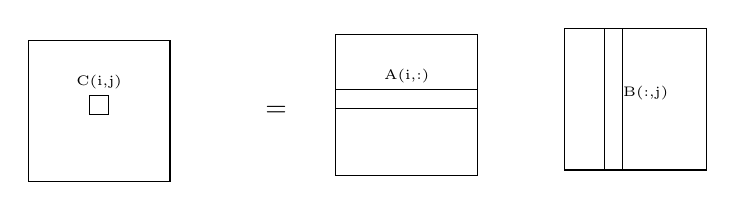
\begin{tikzpicture}[scale=1, every node/.style={transform shape}]
		%%	\tikzstyle{taskr}=[draw=black, minimum height=18mm, minimum width=18mm, anchor=south west, fill=pastelgreen, text=black]
		
		\tikzstyle{taskr}=[draw=black, minimum height=18mm, minimum width=18mm, fill=pastelgreen, text=black]
		
		\tikzstyle{taskrow}=[draw=black, minimum height=2mm, minimum width=18mm, fill=pastelgreen, fill=none, text=black]
		\tikzstyle{taskcol}=[draw=black, minimum height=18mm, minimum width=2mm, fill=pastelgreen, fill=none, text=black]
		
		\tikzstyle{taskrsmall}=[draw=black, minimum height=2mm, minimum width=2mm, fill=none, text=black]
		
		%%	\node(t1) at (0,0) {};
		%%	\node [above right=0cm and 0cm of t1.mid,taskr](T1) {};
		\node [taskr, fill=none] (T1) at (0,0) {};
		\node [taskrsmall] (T2) at (T1.mid) {};
		\node [above] at (T2.mid) {\tiny C(i,j)};
		\node[draw=none, text=black, scale=1] at (2.25,0) {$=$};
		
		\node [right=3cm of T1.mid,taskr, fill=none](T3) {};
		\node[taskrow](T4) at (T3.mid) {};
		\node [above] at (T4.mid) {\tiny A(i,:)};
		
		\node [right=2cm of T3.mid,taskr, fill=none](T5) {};
		\node [right=2.5cm of T3.mid, taskcol](T6) {};
		\node [right] at (T6.mid) {\tiny B(:,j)};
		
		\end{tikzpicture}
	\end{center}
\end{frame}


\begin{frame}{Matrix multiplication: linear combination of columns}
	\begin{itemize}
		\item A column of $C$ is obtained by linear combination of columns of $A$.
	\end{itemize}
	\begin{center}
		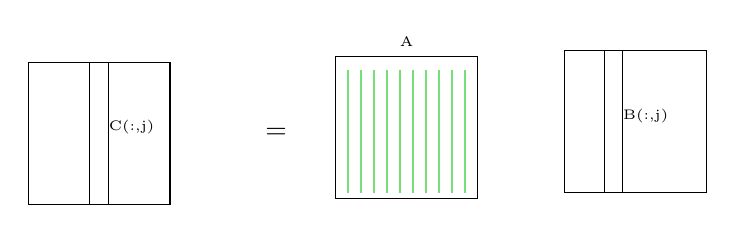
\begin{tikzpicture}[scale=1, every node/.style={transform shape}]
		%%	\tikzstyle{taskr}=[draw=black, minimum height=18mm, minimum width=18mm, anchor=south west, fill=pastelgreen, text=black]
		
		\tikzstyle{taskr}=[draw=black, minimum height=18mm, minimum width=18mm, fill=pastelgreen, text=black]
		
		\tikzstyle{taskrow}=[draw=black, minimum height=2mm, minimum width=18mm, fill=pastelgreen, fill=none, text=black]
		\tikzstyle{taskcol}=[draw=black, minimum height=18mm, minimum width=2mm, fill=pastelgreen, fill=none, text=black]
		
		\tikzstyle{taskrsmall}=[draw=black, minimum height=2mm, minimum width=2mm, fill=none, text=black]
		
		%%	\node(t1) at (0,0) {};
		%%	\node [above right=0cm and 0cm of t1.mid,taskr](T1) {};
		\node [taskr, fill=none] (T1) at (0,0) {};
		\node [taskcol] (T2) at (0,0) {};
		\node [right] at (T2.mid) {\tiny C(:,j)};
		
		\node[draw=none, text=black, scale=1] at (2.25,0) {$=$};
		%%	
		\node [right=3cm of T1.mid,taskr, fill=none](T3) {};
		%%	\node[taskrow](T4) at (T3.mid) {};
		\node [above] at (T3.north) {\tiny A};
		%%	\draw[pastelgreen, thick] (3.1cm, 0.8) -- (3.1cm, -0.75);
		%%	\draw[pastelgreen, thick] (3.2cm, 0.8) -- (3.2cm, -0.75);
		%%	\draw[pastelgreen, thick] (3.3cm, 0.8) -- (3.3cm, -0.75);
		%%	\draw[pastelgreen, thick] (3.45cm, 0.8) -- (3.45cm, -0.75);
		\foreach \x in {1,2,3,4,5,6,7,8,9,10}
		\draw [pastelgreen, thick] (3+0.165* \x, 0.8) -- (3+0.165* \x, -0.75);
		%%  \foreach \y [count=\yi] in {0,...,3}  
		%%  \draw (\x\y)--(\x\yi) (\y\x)--(\yi\x) ;
		
		%%	
		\node [right=2cm of T3.mid,taskr, fill=none](T5) {};
		\node [right=2.5cm of T3.mid, taskcol](T6) {};
		\node [right] at (T6.mid) {\tiny B(:,j)};
		%%	
		\end{tikzpicture}
	\end{center}
\end{frame}

\begin{frame}{Matrix multiplication: linear combination of rows}
	\begin{itemize}
		\item A row of $C$ is obtained by linear combination of rows of $B$.
	\end{itemize}
	\begin{center}
		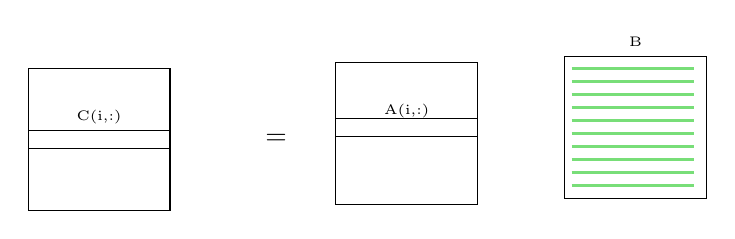
\begin{tikzpicture}[scale=1, every node/.style={transform shape}]
		%%	\tikzstyle{taskr}=[draw=black, minimum height=18mm, minimum width=18mm, anchor=south west, fill=pastelgreen, text=black]
		
		\tikzstyle{taskr}=[draw=black, minimum height=18mm, minimum width=18mm, fill=pastelgreen, text=black]
		
		\tikzstyle{taskrow}=[draw=black, minimum height=2mm, minimum width=18mm, fill=pastelgreen, fill=none, text=black]
		\tikzstyle{taskcol}=[draw=black, minimum height=18mm, minimum width=2mm, fill=pastelgreen, fill=none, text=black]
		
		\tikzstyle{taskrsmall}=[draw=black, minimum height=2mm, minimum width=2mm, fill=none, text=black]
		
		%%	\node(t1) at (0,0) {};
		%%	\node [above right=0cm and 0cm of t1.mid,taskr](T1) {};
		\node [taskr, fill=none] (T1) at (0,0) {};
		\node [taskrow] (T2) at (0,0) {};
		\node [above] at (T2.mid) {\tiny C(i,:)};
		
		\node[draw=none, text=black, scale=1] at (2.25,0) {$=$};
		%%	
		\node [right=3cm of T1.mid,taskr, fill=none](T3) {};
		\node[taskrow](T4) at (T3.mid) {};
		\node [above] at (T3.mid) {\tiny A(i,:)};
		%%	\node [above] at (T3.north) {\tiny A};
		%%	\draw[pastelgreen, thick] (3.1cm, 0.8) -- (3.1cm, -0.75);
		%%	\draw[pastelgreen, thick] (3.2cm, 0.8) -- (3.2cm, -0.75);
		%%	\draw[pastelgreen, thick] (3.3cm, 0.8) -- (3.3cm, -0.75);
		%%	\draw[pastelgreen, thick] (3.45cm, 0.8) -- (3.45cm, -0.75);
		%%	\foreach \x in {1,2,3,4,5,6,7,8,9,10}
		%%		\draw [pastelgreen, thick] (3+0.165* \x, 0.8) -- (3+0.165* \x, -0.75);
		%%  \foreach \y [count=\yi] in {0,...,3}  
		%%  \draw (\x\y)--(\x\yi) (\y\x)--(\yi\x) ;
		
		%%	
		\node [right=2cm of T3.mid,taskr, fill=none](T5) {};
		\node [above] at (T5.north) {\tiny B};
		
		\foreach \x in {1,2,3,4,5,6,7,8,9,10}
		\draw [pastelgreen, thick] (6, -0.75+0.165* \x) -- (7.56, -0.75+0.165* \x);
		
		%%	\node [right=2.5cm of T3.mid, taskcol](T6) {};
		%%	\node [right] at (T6.mid) {\tiny B(:,j)};
		%%	
		\end{tikzpicture}
	\end{center}
	
\end{frame}

\begin{frame}{Matrix multiplication: sum of $n$ matrices}
	\begin{itemize}
		\item Matrix multiplication can also be viewed as sum of $n$ matrices.
	\end{itemize}
	\begin{center}
		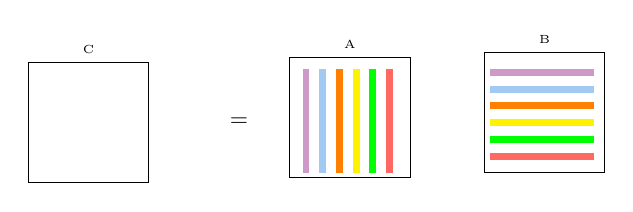
\begin{tikzpicture}[scale=0.85, every node/.style={transform shape}]
		%%	\tikzstyle{taskr}=[draw=black, minimum height=18mm, minimum width=18mm, anchor=south west, fill=pastelgreen, text=black]
		
		\tikzstyle{taskr}=[draw=black, minimum height=18mm, minimum width=18mm, fill=pastelgreen, text=black]
		
		\tikzstyle{taskrow}=[draw=black, minimum height=2mm, minimum width=18mm, fill=pastelgreen, fill=none, text=black]
		\tikzstyle{taskcol}=[draw=black, minimum height=18mm, minimum width=2mm, fill=pastelgreen, fill=none, text=black]
		
		\tikzstyle{taskrsmall}=[draw=black, minimum height=2mm, minimum width=2mm, fill=none, text=black]
		
		%%	\node(t1) at (0,0) {};
		%%	\node [above right=0cm and 0cm of t1.mid,taskr](T1) {};
		\node [taskr, fill=none] (T1) at (0,0) {};
		%%	\node [taskrow] (T2) at (0,0) {};
		\node [above] at (T1.north) {\tiny C};
		
		\node[draw=none, text=black, scale=1] at (2.25,0) {$=$};
		%%	
		\node [right=3cm of T1.mid,taskr, fill=none](T3) {};
		%%	\node[taskrow](T4) at (T3.mid) {};
		%%	\node [above] at (T3.mid) {\tiny A(i,:)};
		\node [above] at (T3.north) {\tiny A};
		%%	\draw[pastelgreen, thick] (3.1cm, 0.8) -- (3.1cm, -0.75);
		%%	\draw[pastelgreen, thick] (3.2cm, 0.8) -- (3.2cm, -0.75);
		%%	\draw[pastelgreen, thick] (3.3cm, 0.8) -- (3.3cm, -0.75);
		%%	\draw[pastelgreen, thick] (3.45cm, 0.8) -- (3.45cm, -0.75);´
		%%	  \foreach \x/\xtext in {0,...,3,2.72 / e} 
		\foreach \x/\y in {1/pastelviolet, 2/babyblueeyes, 3/orange, 4/yellow, 5/green, 6/pastelred}
		\draw [\y, line width = 2.5] (3+0.25* \x, 0.8) -- (3+0.25* \x, -0.75);
		%%  \foreach \y [count=\yi] in {0,...,3}  
		%%  \draw (\x\y)--(\x\yi) (\y\x)--(\yi\x) ;
		
		%%	
		\node [right=2cm of T3.mid,taskr, fill=none](T5) {};
		\node [above] at (T5.north) {\tiny B};
		
		\foreach \x/\y in {1/pastelviolet, 2/babyblueeyes, 3/orange, 4/yellow, 5/green, 6/pastelred}
		\draw [\y, line width = 2.5] (6, 1-0.25* \x) -- (7.56, 1-0.25* \x);
		
		%%	\node [right=2.5cm of T3.mid, taskcol](T6) {};
		%%	\node [right] at (T6.mid) {\tiny B(:,j)};
		%%	
		\end{tikzpicture}
	\end{center}

	\begin{center}
		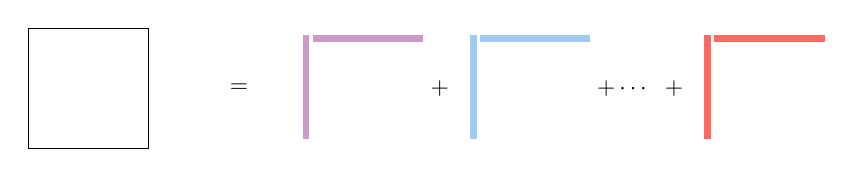
\begin{tikzpicture}[scale=0.85, every node/.style={transform shape}]
		%%	\tikzstyle{taskr}=[draw=black, minimum height=18mm, minimum width=18mm, anchor=south west, fill=pastelgreen, text=black]
		
		\tikzstyle{taskr}=[draw=black, minimum height=18mm, minimum width=18mm, fill=pastelgreen, text=black]
		
		
		%%	\node(t1) at (0,0) {};
		%%	\node [above right=0cm and 0cm of t1.mid,taskr](T1) {};
		\node [taskr, fill=none] (T1) at (0,0) {};
		%%	\node [taskrow] (T2) at (0,0) {};
		%%	\node [above] at (T1.north) {\tiny C};
		
		\node[draw=none, text=black] at (2.25,0) {$=$};
		
		\draw [pastelviolet, line width = 2.5] (3+0.25, 0.8) -- (3+0.25, -0.75);
		\draw [pastelviolet, line width = 2.5] (3+0.35, 1-0.25) -- (5, 1-0.25);
		\node[draw=none, text=black] at (5.25,0) {$+$};
		
		\draw [babyblueeyes, line width = 2.5] (2.5+3+0.25, 0.8) -- (2.5+3+0.25, -0.75);
		\draw [babyblueeyes, line width = 2.5] (2.5+3+0.35, 1-0.25) -- (2.5+5, 1-0.25);
		\node[draw=none, text=black] at (2.75+5.25,0) {$+\cdots$};
		
		\node[draw=none, text=black] at (3.5+5.25,0) {$+$};
		\draw [pastelred, line width = 2.5] (9.25, 0.8) -- (9.25, -0.75);
		\draw [pastelred, line width = 2.5] (9.35, 1-0.25) -- (9.35+1.65, 1-0.25);
		
		%%	
		%%	\node [right=3cm of T1.mid,taskr, fill=none](T3) {};
		%%	%%	\node[taskrow](T4) at (T3.mid) {};
		%%	%%	\node [above] at (T3.mid) {\tiny A(i,:)};
		%%	\node [above] at (T3.north) {\tiny A};
		%%	%%	\draw[pastelgreen, thick] (3.1cm, 0.8) -- (3.1cm, -0.75);
		%%	%%	\draw[pastelgreen, thick] (3.2cm, 0.8) -- (3.2cm, -0.75);
		%%	%%	\draw[pastelgreen, thick] (3.3cm, 0.8) -- (3.3cm, -0.75);
		%%	%%	\draw[pastelgreen, thick] (3.45cm, 0.8) -- (3.45cm, -0.75);´
		%%	%%	  \foreach \x/\xtext in {0,...,3,2.72 / e} 
		%%	\foreach \x/\y in {1/pastelviolet, 2/babyblueeyes, 3/orange, 4/yellow, 5/green, 6/pastelred}
		%%	\draw [\y, line width = 2.5] (3+0.25* \x, 0.8) -- (3+0.25* \x, -0.75);
		%%	%%  \foreach \y [count=\yi] in {0,...,3}  
		%%	%%  \draw (\x\y)--(\x\yi) (\y\x)--(\yi\x) ;
		%%	
		%%	%%	
		%%	\node [right=2cm of T3.mid,taskr, fill=none](T5) {};
		%%	\node [above] at (T5.north) {\tiny B};
		%%	
		%%	\foreach \x/\y in {1/pastelviolet, 2/babyblueeyes, 3/orange, 4/yellow, 5/green, 6/pastelred}
		%%	\draw [\y, line width = 2.5] (6, 1-0.25* \x) -- (7.56, 1-0.25* \x);
		%%	
		%%	%%	\node [right=2.5cm of T3.mid, taskcol](T6) {};
		%%	%%	\node [right] at (T6.mid) {\tiny B(:,j)};
		%%	%%	
		\end{tikzpicture}
	\end{center}
	
	
\end{frame}


\begin{frame}{Matrix multiplication: recursive calls on submatrices}
	\begin{itemize}
		\item Matrix is divided into 2$\times$2 blocks
	\end{itemize}
	%%\begin{pmatrix}
	%%	1 & 2 & 3\\
	%%	a & b & c
	%%\end{pmatrix}
	
	\begin{align*}
	\begin{pmatrix}
	C_{11} & C_{12} \\
	C_{21} & C_{22}
	\end{pmatrix}
	&
	=
	\begin{pmatrix}
	A_{11} & A_{12} \\
	A_{21} & A_{22}
	\end{pmatrix}
	\begin{pmatrix}
	B_{11} & B_{12} \\
	B_{21} & B_{22}
	\end{pmatrix}
	\end{align*}
	
	\begin{align*}
	C_{11} &= A_{11}B_{11} + A_{12}B_{21}\\
	C_{12} &= A_{11}B_{12} + A_{12}B_{22}\\
	C_{21} &= A_{21}B_{11} + A_{22}B_{21}\\
	C_{22} &= A_{21}B_{12} + A_{22}B_{22}\\
	\end{align*}
\end{frame}


\begin{frame}{Matrix multiplication: recursive calls on submatrices}
	Operation count recurrence,
	\begin{align*}
	T(n) &= 8T\Big(\frac{n}{2}\Big) + \mathcal{O}(n^2)\\
	T(n) &= 1
	\end{align*}
	Here $\mathcal{O}(n^2)$ refers that $\exists c\in\mathbb{N}$ such that this term is less than or equal to $cn^2$ for every $n$.
	\medskip
	
	
	After solving, we obtain $T(n) = \mathcal{O}(n^3)$.
\end{frame}


\subsection{Strassen's Matrix Multiplication}
	\begin{frame}{Table of Contents}		
	\tableofcontents[currentsection,currentsubsection] 		
	\end{frame}


\begin{frame}{Matrix multiplication: Strassen's algorithm}
	\begin{align*}
	\begin{pmatrix}
	C_{11} & C_{12} \\
	C_{21} & C_{22}
	\end{pmatrix}
	&
	=
	\begin{pmatrix}
	A_{11} & A_{12} \\
	A_{21} & A_{22}
	\end{pmatrix}
	\begin{pmatrix}
	B_{11} & B_{12} \\
	B_{21} & B_{22}
	\end{pmatrix}
	\end{align*}
	
	\begin{minipage}{0.45\columnwidth}
		\begin{align*}\small
		M_1 &= (A_{11} + A_{22})(B_{11}+B_{22})\\
		M_2 &= (A_{21} + A_{22})B_{11}\\
		M_3 &= A_{11} (B_{12}-B_{22})\\
		M_4 &= A_{22} (B_{21}-B_{11})\\
		M_5 &= (A_{11} +A_{12})B_{22}\\
		M_6 &= (A_{21}-A_{11})(B_{11} +B_{12})\\
		M_7 &= (A_{12}-A_{22})(B_{21} + B_{22}) 
		\end{align*}
	\end{minipage}
	\hfill
	\begin{minipage}{0.45\columnwidth}
		\begin{center}
			\begin{align*}
			C_{11} &= M_1 + M_4 -M_5 +M_7\\
			C_{12} &= M_3 + M_5\\
			C_{21} &= M_2 + M_4\\
			C_{22} &= M_1 -M_2 + M_3 + M_6
			\end{align*}
		\end{center}
	\end{minipage}
	
\end{frame}



\begin{frame}{Matrix multiplication: Strassen's algorithm}
	Operation count recurrence,
	\begin{align*}
	T(n) &= 7T\big(\frac{n}{2}\big) + \mathcal{O}(n^2)\\
	T(n) &= 1
	\end{align*}
	After solving, we obtain $T(n) = \mathcal{O}(n^{\log_2 7})$.\\
	$\qquad\qquad\qquad\qquad\qquad\log_2 7 \approx 2.81$
	%% \mathcal{O}(n^{2.81})$.
	\begin{block}{Open questions}
		\begin{itemize}
			\item Is there a way to perform matrix multiplication in less number of operations than this algorithm?
			\item What is the minimum number of operations to perform matrix multiplication?
		\end{itemize}
	\end{block}
\end{frame}
\section{Algorithms}
\begin{frame}
	\frametitle{Table of Contents}
	\tableofcontents[currentsection,hideallsubsections]
\end{frame}
\begin{frame}[fragile]{Analysis of traditional matrix multiplication algorithm}
	\begin{verbatim}
	//implements C=C+AB
	for i=1 to n
	  for j=1 to n
	    for k=1 to n
	      C(i,j) = C(i,j) + A(i,k) * B(k,j);
	\end{verbatim}
	%%\only<2>{\begin{verbatim}
	%%	//implements C =C+AB
	%%	for i=1 to n
	%%	// read row i of A into fast memory  (total n read) 
	%%	for j=1 to n
	%%	// read row i of C into fast memory (total n read)
	%%	// read column j of B into fast memory (total n read)
	%%	for k=1 to n
	%%	  C(i,j) = C(i,j) + A(i,k) * B(k,j);
	%%	  // write row i of C back to slow memory (total n read)
	%%	\end{verbatim}
	%%$n^2 + 3n^2$ reads/writes combined dominates $2n^3$ computations}
\end{frame}

\begin{frame}[fragile]{Analysis of traditional matrix multiplication algorithm}
	\begin{verbatim}
	//implements C=C+AB
	for i=1 to n
	 for j=1 to n
	  // read row i of C into fast memory (total n^2 reads)
	  for k=1 to n
	  	// read row i of A into fast memory  (total n^3 reads) 
	    // read column j of B into fast memory (total n^3 reads)
	    C(i,j) = C(i,j) + A(i,k) * B(k,j);
	  // write row i of C back to slow memory (total n^2 writes)
	\end{verbatim}
	\medskip
	$2n^3 + 2n^2$ reads/writes combined dominates $2n^3$ computations.
\end{frame}

\begin{frame}{Tiled matrix multiplication}
	\begin{itemize}
		\item A, B, C are  $n/b \times n/b$ matrices of $b \times b$ subblocks
		\item $3$ $b \times b$ blocks fit in the fast memory
	\end{itemize}
\vfill

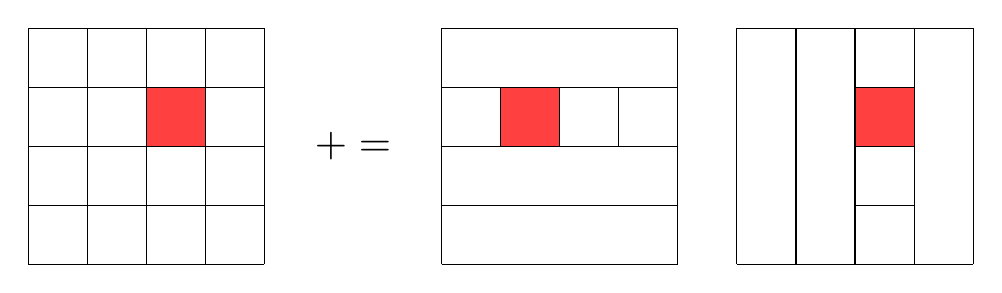
\begin{tikzpicture}[scale=0.75, every node/.style={transform shape}]
\foreach \x in {0,1,2,3,4}
{ 
	\draw  (0,\x) -- (4,\x);
	\draw (\x, 0) -- (\x, 4);
}

\node[draw=none, text=black, scale=2] at (5.5,2) {$+=$};
\draw [fill=red!75] (2,2) -- ++ (1,0) -- ++(0,1) --++(-1,0) -- cycle;
%	\draw[blue,fill=pastelgreen] (0,0) -- node [below, scale=6, black] {Vector}++(-\rectx,0) -- ++(0,\recty) -- ++(\rectx, 0) -- cycle;



\foreach \x in {0,1,2,3,4}
	\draw  (7,\x) -- (11,\x);
	
\draw (7,0) -- (7,4);
\draw (11,0) -- (11,4);

\foreach \x in {0,1,2,3,4}
\draw  (7+\x,2) -- (7+\x,3);

\draw [fill=red!75] (8,2) -- ++ (1,0) -- ++(0,1) --++(-1,0) -- cycle;

\foreach \x in {0,1,2,3,4}
\draw  (12+\x,0) -- (12+\x,4);

\draw (12,0) -- (16,0);
\draw (12,4) -- (16,4);

\foreach \x in {0,1,2,3,4}
\draw  (14,\x) -- (15,\x);

\draw [fill=red!75] (14,2) -- ++ (1,0) -- ++(0,1) --++(-1,0) -- cycle;


	
%		\draw (\x, 0) -- (\x, 4);

\end{tikzpicture}


\end{frame}
\begin{frame}[fragile]{Tiled matrix multiplication}
%	\vspace*{-0.25cm}
%	//Consider A, B, C to be n/b X n/b matrices of b x b subblocks
%	//Asumme 3 b x b blocks fit in fast memory
	\begin{verbatim}
	for i=1 to n/b
	  for j=1 to n/b
	    // read block C(i,j) into fast memory 
	    // (total b^2 * n/b * n/b = n^2 reads)
	    for k=1 to n/b
	      // read block A(i,k) into fast memory 
	      // (total b^2 * n/b * n/b * n/b = n^3/b reads)
	      // read block B(k,j) into fast memory 
	      // (total b^2 * n/b * n/b * n/b = n^3/b reads)
	      //perform block matrix multiplication
	      C(i,j) = C(i,j) + A(i,k) * B(k,j);
	    // write block C(i,j) into fast memory 
	    // (total b^2 * n/b * n/b = n^2 writes)
	\end{verbatim}
	\medskip
	$\frac{2n^3}{b} + 2n^2$ reads/writes $<<$ $2n^3$ computations.
\end{frame}

\begin{frame}{Amount of volume in matrix multiplication }
	\begin{itemize}
		\item Let M be the size of the fast memory, make b as large as possible, 3$b^2 \le M$
		\item Number of reads/writes $\ge2\sqrt{3}n^3/\sqrt{M} + 2n^2$
	\end{itemize}
	\vfill
	\brown{Question}: Is this optimal?

\end{frame}
\begin{frame}[fragile]{Assignment 1 -- deadline Sept. 21}
	\begin{verbatim}
for i=1 to m
  for j=1 to n
    for k=1 to l
      C(i,j) = C(i,j) + A(i,k) * B(k,j);
\end{verbatim}
Here $A \in\mathbb{R}^{m \times \ell}$, $B \in\mathbb{R}^{\ell \times n}$, and  $C$ $\in$ $\mathbb{R}^{m \times n}$. The computation is performed with infinite precision.

\brown{Questions:}
\begin{enumerate}
	\item {\small Prove that all the $6$ permutations of the loops produce the same output.}
	\item {\small Compute the number of cache misses for each permutation of the loops. All matrices are stored in the row-major order in the slow memory. Size of each cache line is $L$ and the cache capacity $< <$ $\min(m,n,\ell)$. Assume that the cache is fully associative and the least recently used (LRU) strategy is employed to evict a cache line.}
\end{enumerate} 
\end{frame}

%		\item $C= AB$, where $A \in\mathbb{R}^{m \times k}$, $B \in\mathbb{R}^{k \times n}$, and  $C$ $\in$ $\mathbb{R}^{m \times n}$.
\section{Communication bounds}
\begin{frame}{Table of Contents}
	\tableofcontents[currentsection,hideallsubsections]
\end{frame}
\begin{frame}{Approach to obtain communication lower bounds}
	
			\begin{itemize}
				\item Loomis-Whitney inequalitiy: for $d-1$ dimensional projections
				\begin{itemize}
					\item For the $2$d object $G$, $ Area(G) \le \phi_x \phi_y$
					\item For the $3$d object $H$, $Volume(H) \le \sqrt{\phi_{xy}\phi_{yz}\phi_{xz}}$
					%%		\item $2$-dimensional object $A$ and its $1$-dimensional projections are $\phi_x$ and $\phi_y$, then $\phi_x \phi_y \ge Area(A)$
					%%		\item $3$-dimensional object $B$ and its $2$-dimensional projections are $\phi_{xy}$, $\phi_{yz}$ and $\phi_{xz}$, then $(\phi_{xy}\phi_{yz}\phi_{xz})^\frac{1}{2} \ge Volume(B)$
				\end{itemize}
			\end{itemize}

			\begin{center}
				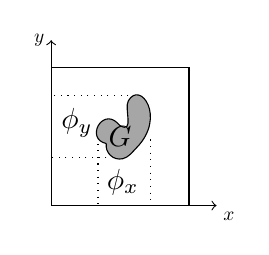
\begin{tikzpicture}[scale=0.35, every node/.style={transform shape}]
				\draw (0,0) -- ++(5,0) -- ++(0, 5) -- ++(-5,0) -- cycle;
				\draw [<->] (0,6) -- (0,0) -- (6,0);
				\node [below right, scale=2] at (6,0) {$x$};
				\node [left, scale=2] at (0,6) {$y$};
				
				\draw [fill=gray!70] (2,2.25) to [curve through={(2.4,3) .. (2.5,2.9) .. (2.8,3.8) .. (3.1,2.1) .. (2.6,1.7)}] (2,2.25);
				
				\node [scale=3] at (2.5,2.5) {$G$};
				\draw [dotted] (1.7,2.25) -- (1.7,0);
				\draw [dotted] (3.6,2.4) -- (3.6,0);
				
				\node[above, scale=3] at (2.6,0) {$\phi_x$};
				
				\draw [dotted] (2,1.75) -- (0,1.75);
				\draw [dotted] (2.8,4) -- (0,4);
				
				\node[right, scale=3] at (0,3) {$\phi_y$};
				\end{tikzpicture}
				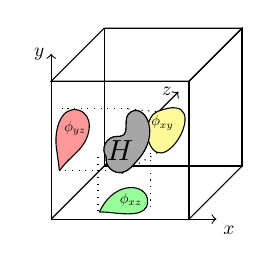
\begin{tikzpicture}[scale=0.35, every node/.style={transform shape}]
				\draw (0,0) -- ++(5,0) -- ++(0, 5) -- ++(-5,0) -- cycle;
				\draw (0,5,0) -- ++(0,0, -5) -- ++(5,0,0) -- ++(0,0,5) -- cycle;
				\draw (5,0,0) -- ++(0,0,-5) -- ++(0,5,0) -- ++(0,0,5) -- cycle;
				\draw (0,0,-5) -- ++(5,0,0) -- ++(0,5,0) -- ++(-5,0,0) -- cycle;
				\draw [<->] (0,6) -- (0,0) -- (6,0);
				\draw [->] (0,0,0) -- (0,0,-12);
				\node [left, scale=2, rotate=0] at (0,0,-12) {$z$};
				\node [below right, scale=2] at (6,0) {$x$};
				\node [left, scale=2] at (0,6) {$y$};
				
				\draw [fill=gray!70] (2,2.25) to [curve through={(2.4,3) .. (2.5,3) .. (2.8,3.8) .. (3.1,2.1) .. (2.6,1.7)}] (2,2.25);
				
%				\node [scale=2] at (2.5,2.5) {$G$};
				\draw [dotted] (1.7,2.25) -- (1.7,0.2);
				\draw [dotted] (3.6,2.4) -- (3.6,0.3);
				
				\draw [fill=green!40] (1.75,0.25) to [curve through={(1.8, 0.35) .. (3.5, 0.65) .. (2,0.25)}] (1.75,0.25);
				\node[above, scale=1.5] at (2.6,0,-0.75) {$\phi_{xz}$};
				
				\draw [dotted] (2,1.75) -- (0.3,1.75);
				\draw [dotted] (2.8,4) -- (0.385,4);
				
				\draw [fill=red!40] (0.3, 1.75) to [curve through={(0.5,2) .. (1, 2.5) .. (1,3.95) .. (0.2, 2.5)}] (0.3,1.75);
				\node[right, scale=1.5] at (0,3, -0.75) {$\phi_{yz}$};
				
				\draw [fill=yellow!40] (3.85,3.9) to [curve through={(3.7,3.8) .. (3.5,3.4) .. (3.45,3.2)}] (3.85, 3.9);
				\node [scale=1.5] at (3.65,3.1,-1) {$\phi_{xy}$};
				\draw [dotted] (2.8,4) -- (3.8,3.9);
				\draw [dotted] (2.56,1.65) -- (4,2.5);
				
				\draw [fill=gray!70] (2,2.25) to [curve through={(2.4,3) .. (2.5,3) .. (2.8,3.8) .. (3.1,2.1) .. (2.6,1.7)}] (2,2.25);
				
				\node [scale=3] at (2.5,2.5) {$H$};
				\end{tikzpicture}
			\end{center}

		\begin{itemize}
			\item H\"{o}lder-Brascamp-Lieb (HBL) inequality -- generalization for arbitrary dimensional projections
			\begin{itemize}
				\item Provide exponent for each projection
				
			\end{itemize}
		\end{itemize}
\end{frame}


\begin{frame}{Number of iterations with a phases of $R$ reads ($\neq M$)}
	
	\begin{theorem}
		During a phase of $R$ reads with memory $M$, the number of computed iterations is bounded by
		$$
		F_{M+R} \leq \left(\frac{1}{3}(M+R)\right)^{3/2}
		$$    
	\end{theorem}
	
	Maximize $F_{M+R}$ constrained by:
	$$\left\{
	\begin{array}[c]{l}
	F_{M+R} \leq \sqrt{N_A N_B N_C}\\
	0\leq N_A, N_B, N_C\\
	N_A+N_B+N_C \leq M+R
	\end{array}
	\right.
	$$
	Using Lagrange multipliers, maximal value obtained when $N_A=N_B=N_C$
	\vfill
\end{frame}

\begin{frame}[fragile]{Selection of $R$}
	\begin{verbatim}
	for i=1 to m
	  for j=1 to n
	    for k=1 to l
	      C(i,j) = C(i,j) + A(i,k) * B(k,j);
	\end{verbatim}


	$\textnormal{Total number of iterations in one phase:~~}    F_{M+R} \leq \left(\frac{1}{3}(M+R)\right)^{3/2}$
  
  \vfill
	
	Total volume of reads:
	$$V_{\textnormal{read}} \geq \left\lfloor \frac{mn\ell}{F_{M+R}} \right\rfloor \cdot R \geq \left( \frac{mn\ell}{F_{M+R}} -1 \right) \cdot R $$
	Valid for all values of $R$, maximized when $R=2M$:
	$$V_{\textnormal{read}} \geq 2mn\ell/\sqrt{M} -2M$$

	
\end{frame}
\begin{frame}{Communication bounds}
	
	$$V_{\textnormal{read}} \geq 2mn\ell/\sqrt{M} -2M$$
	
	All elements of the output matrix are in the slow memory in the end. Each element of $C$ is written at least once: $V_{\textnormal{write}} \geq mn$\\
	
	\begin{theorem}
		The total volume of I/Os is bounded by:
		$$
		V_{I/O} \geq  2mn\ell/\sqrt{M} + mn -2M
		$$
	\end{theorem}
	
\begin{block}{Our tiled algorithm (explained previously)}
	\begin{itemize}
		\item With square matrices, total number of reads/writes $\ge2\sqrt{3}n^3/\sqrt{M} + 2n^2$
		\item How far it is from the lower bound?
	\end{itemize}

\end{block}

\end{frame}
\begin{frame}{Structure of the optimal algorithm (attaining the same constant for the leading term)}
Consider the following algorithm sketch:
\begin{itemize}
	\item Partition $C$ into blocks of size $(\sqrt{M}-1)\times (\sqrt{M}-1)$
	\item Partition $A$ into block-columns of size $(\sqrt{M}-1)\times 1$
	\item Partition $B$ into block-rows of size $1 \times (\sqrt{M}-1)$
	\item For each block $C_b$ of $C$:
	\begin{itemize}
		\item Load the corresponding blocks of $A$ and $B$ on after the
		other
		\item For each pair of blocks $A_b, B_b$, compute $C_b \gets C_b
		+A_b B_b$
		\item When all computations for $C_b$ are performed, write back $C_b$
	\end{itemize}
\end{itemize}

\vfill
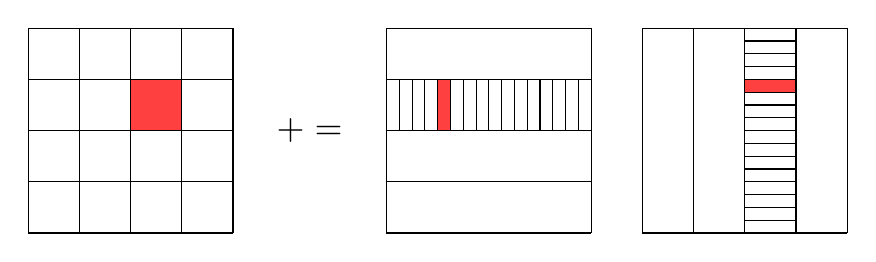
\begin{tikzpicture}[scale=0.65, every node/.style={transform shape}]
\foreach \x in {0,1,2,3,4}
{ 
	\draw  (0,\x) -- (4,\x);
	\draw (\x, 0) -- (\x, 4);
}

\node[draw=none, text=black, scale=2] at (5.5,2) {$+=$};
\draw [fill=red!75] (2,2) -- ++ (1,0) -- ++(0,1) --++(-1,0) -- cycle;
%	\draw[blue,fill=pastelgreen] (0,0) -- node [below, scale=6, black] {Vector}++(-\rectx,0) -- ++(0,\recty) -- ++(\rectx, 0) -- cycle;



\foreach \x in {0,1,2,3,4}
\draw  (7,\x) -- (11,\x);

\draw (7,0) -- (7,4);
\draw (11,0) -- (11,4);

\foreach \x in {0,0.25, 0.5, 0.75, 1, 1.25, 1.5, 1.75, 2, 2.25, 2.5, 2.75, 3, 3.25, 3.5, 3.75,4}
\draw  (7+\x,2) -- (7+\x,3);

\draw [fill=red!75] (8,2) -- ++ (0.25,0) -- ++(0,1) --++(-0.25,0) -- cycle;

\foreach \x in {0,1,2,3,4}
\draw  (12+\x,0) -- (12+\x,4);

\draw (12,0) -- (16,0);
\draw (12,4) -- (16,4);

\foreach \x in {0,0.25, 0.5, 0.75, 1, 1.25, 1.5, 1.75, 2, 2.25, 2.5, 2.75, 3, 3.25, 3.5, 3.75,4}
\draw  (14,\x) -- (15,\x);

\draw [fill=red!75] (14,2.75) -- ++ (1,0) -- ++(0,0.25) --++(-1,0) -- cycle;



%		\draw (\x, 0) -- (\x, 4);

\end{tikzpicture}


%Questions:
%\begin{enumerate}
%	\item Write a proper algorithm following these directions
%	\item Compute the number of read and write operations
%	\item Conclude that the algorithm is asymptotically optimal
%\end{enumerate}

\end{frame}


%\subsection{Another approach}

\begin{frame}{Another approach to computer communication bound}
	\textbf{Red-Blue pebble game (Hong and Kung, 1981)}:
	\begin{itemize}
		\item \darkred{Red pebbles}: limited number $S$ (slots in fast memory)
		\item \darkblue{Blue pebbles}: unlimited number, only for slow memory
	\end{itemize}
	\vfill
	
	\structure{Rules:}
	\begin{enumerate}[(1)]
		\item A \darkred{red} pebble may be placed on a vertex that has a \darkblue{blue} pebble.
		\item A \darkblue{blue} pebble may be placed on a vertex that has a \darkred{red} pebble.
		\item If all predecessors of a vertex $v$ have a \darkred{red} pebble, a \darkred{red}
		pebble may be placed on $v$.
		\item A pebble (\darkred{red} or \darkblue{blue}) may be removed at
		any time.
		\item No more than $S$ \darkred{red} pebbles may be used at any time.
		\item A \darkblue{blue} pebble can be placed on an input vertex at any time
	\end{enumerate}
	\vfill
	
	\structure{Objective:} put a \darkred{red} pebble on each target (not necessary
	simultaneously) using a minimum rules 1 and 2 (I/O operations)
	\vfill
\end{frame}

\begin{frame}
	\frametitle{Example: FFT graph}
	
	\centerline{\includegraphics[width=0.68\linewidth]{FFT.pdf}}
	{\footnotesize $k$ levels,$n=2^{k}$ vertices at each level}\\
	
	Minimum number $S$ of \darkred{red} pebbles ? \\
	How many I/Os for this minimum number $S$  ?
\end{frame}


\end{document} 